\documentclass{article}
\usepackage{xcolor}
\usepackage{minted}

% Author info %
\title{AQA A Level Computer Science NEA}
\date{2023}
\author{Luka Warren}

% Code snippet config %
\setminted{fontsize=\footnotesize}

% For images %
\usepackage{graphicx}

% Page layout %
\usepackage[margin=1.0in]{geometry}
\setlength{\fboxsep}{1.5em}
\addtolength{\footnotesep}{5mm}
\usepackage[hang]{footmisc}
\setlength{\footnotemargin}{4mm}

\begin{document}

	% Title page %
	\maketitle
	\pagenumbering{gobble}
	\tableofcontents
	\newpage
	\pagenumbering{arabic}
	
	% Page breaks %
	\AddToHook{cmd/section/before}{\clearpage}
	% \AddToHook{cmd/subsection/before}{\clearpage} %
	
	\section{Analysis}
	
	\subsection{Background}
	There exists online many popular "remixes"  where someone has taken an existing song and distorted it, usually by adjusting its speed, bass and pitch, to achieve a desired effect. Often these versions of the song are preferred to the originals when used to accompany short-form content on video-sharing sites such as TikTok. For example,  the song "Money Trees" by Kendrick Lamar has 120 million views on YouTube  in its original form, but also a sizeable 1.6 million views on one "TikTok remix" alone, and indeed on TikTok itself it is rare to hear the original version.
	
	\paragraph{}
	As such it can be seen that there exists a large audience of people who enjoy listening to altered versions of popular songs. However, the most popular music listening programs, including Spotify and YouTube music, provide no mechanism for manually altering songs by one's self. Whilst there exists ready-made "remixes" by others, there are no mainstream programs which allow a user to "remix" a song in real-time as it is being listened to. This presents two main problems:
	
	\begin{itemize}
		\item Many songs do not have any accompanying "remixes" to satisfy a user's need
		\item The barrier to entry for creating a "remix" prevents easy and user-friendly experimentation
	\end{itemize}
	
	\paragraph{}
	It is therefore the aim of this coursework to create a system to allow users to "remix" songs in real-time as they listen to them. Such a system would allow for comprehensible, user-friendly experimentation, removing the above barrier to entry, whilst providing a mechanism to alter the sound of any arbitrary audio, removing the need to rely on other's work.
	
	\paragraph{}
	However, a system can only be comprehensible and user-friendly if the exact needs of the users themselves are known, and so first a representative sub-section of the user-base must be interviewed.
	
	\subsection{Collection of Data}
	A number of interviews were conducted with peers that self-reported to enjoy listening to song "remixes". Below is a brief summary of the questions asked and the relevant responses.
	
	\paragraph{Question 1 - Why do you sometimes prefer a song's remix?}
	\subparagraph{Student 1}
	Videos on TikTok are only about 30 seconds long. It's good to speed up a song because otherwise you couldn't enjoy the full chorus.
	\subparagraph{Student 2}
	I'm not sure really - I think I prefer it when a song has more bass than usual, and I like how distorted it sounds.
	\subparagraph{Student 3}
	I like watching remixes on YouTube because when they visualise the music it always looks very cool.
	
	\paragraph{Question 2 - How does a remix typically differ from the original song?}
	\subparagraph{Student 1}
	Usually they're faster and I guess that makes them higher-pitched too.
	\subparagraph{Student 2}
	They have more bass and are slowed down a bit. They have a bit of an echo {[effect]} too, and sometimes also they add noise to make it more relaxing. Even the volume is different.
	\subparagraph{Student 3}
	A remix usually has a different speed and is higher or lower than the original.
	
	\paragraph{Question 3 - What features would you like in a real-time audio editing program to assist in "remixing" music?}
	\subparagraph{Student 1}
	I'm not really good with editing so hopefully it would be easy to use. I'd probably only want to apply the same effect every time so there should be a way to help me with that.
	\subparagraph{Student 2}
	I'd like to be able to apply it to my entire music collection because that way all my songs could have the same effects applied. In other words I'd like to apply it to my music playlist.
	\subparagraph{Student 3}
	I think it would be cool to change the speed of songs and change the bass and treble. My car stereo can do that and it's really interesting to play with.


	\subsection{Interview Interpretation}
	\subsubsection{Frequencies}
	Through the interviews it was understood that the ability to modify certain frequency ranges was desirable, in order to affect both the bass and treble. Typically, there are two main ways of doing this:
	\begin{itemize}
		\item Applying a low-pass or high-pass filter to broadly modify the frequencies represented
		\item Modifying the incoming audio in its frequency domain using a Fourier Transform, then converting it back to the time domain using an Inverse Fourier Transform
	\end{itemize}
	Whilst applying a low or high pass filter is a very inexpensive operation, it does not provide exact control over the frequencies modified. Hence in order to best be able to manipulate frequencies, a Fourier Transform must be used.  This is not a computationally trivial task and so every effort must be made to ensure that the program created can still run fast enough to be real-time on typical high school hardware, so as not to increase the barrier of entry, as this would go against the intention of the project.
	
	\subsubsection{Playback Speed}
	The system must also be able to alter the playback speed, as this feature was highly requested. However, again this must not conflict with the real-time requirements of the system on modest high school hardware. In other words, the adjusting of playback speed should not demand a significant computational overhead (or ideally any overhead at all).
	
	\subsubsection{Other Audio Effects}
	Student 2 mentioned "remixes" often contain an "echo" or additional "noise", and so in order to avoid limiting the program to merely changing a song's speed or frequency response, it should also allow the user to apply various audio effects, including but not limited to the ones above. In order to maximise the ease of experimentation, as is desired, the effects should be easily configurable.
		
	\subsubsection{Visualisation}
	As the program is already meant to perform a Fourier Transform on the incoming audio data, it will thus already have a representation of the audio in frequency-space. Hence it would be trivial to display this data graphically so as to provide an audio visualisation feature that is, computationally, essentially free. It is hoped that by providing visual feedback to the audio as it is edited, the effects of, for example, adjusting the bass, will be easy to see and thus the processing the software is carrying out will be easy to comprehend. 
	
	\subsection{Fourier Technical Analysis}
	As mentioned above, in section 1.3.1, it is essential to use a Fourier Transform to be able to modify the incoming audio in frequency-space (for example to provide a "bass-boost"). However, the primary concern is if this algorithm can be carried out fast enough to be able to process audio in real-time.
	
	\paragraph{}
	The primary method for computing Fourier Transforms efficiently is using a Fast Fourier Transform (FFT), which is itself a subset of the Discrete Fourier Transform (DFT). DFTs operate on discrete packets of data, such as audio samples, as opposed to continuous waves, and are hence ideal for this project. Because of the various mathematical tricks used in FFTs, they reduce the time-complexity of computing DFTs from \(O(N^2)\) to \(O(N\log{N})\), providing the performance this project needs (as when dealing with large audio samples N will typically be large).
	
	\paragraph{}
	The most popular FFT algorithm is the "Cooley-Turkey" algorithm, which recursively breaks down its input into two halves. The only limitation of  this approach is that the input data size must generally be a power of two, but as the program should have control over how much data it processes at a time, this should not be an issue.
	
	\paragraph{}
	The formal definition of a DDT may look daunting:
	\[
	X_k = \sum_{n=0}^{N-1} x_n e^{-i2\pi k n/N} 
	\]
	However, a Fourier Transform is essentially just a process to convert a signal into its constituent sine waves. For example, a very basic song may be composed of a number of sine waves with low frequencies (i.e. the bass) plus many higher frequency waves that combine to form the vocals and instruments. Each frequency in an FFT has a corresponding amplitude (volume) and phase (position in time). By adjusting the amplitudes, the relative volumes of a song's frequencies can be modified at will.
	
	\paragraph{}
	It therefore appears that the issue of manipulating frequencies in the coursework should be technically possible, providing performance is maximised by using a Cooley-Turkey FFT.

	\subsection{Programming Language  and Performance Technical Analysis}
	Before embarking on a project design, an appropriate programming language must be chosen. By considering the project requirements it is apparent that two main groups of languages will likely prove insufficient.
	
	\paragraph{Interpreted Languages}
	Languages such as Python and Ruby, whilst intuitive and easy to use, may not provide sufficient CPU performance to easily allow the system to be real-time. Most music typically has two channels, each at a sample rate of around 44,000 Hz, meaning the system must process roughly 88,000 floating point numbers per second at minimum. This number can quickly grow if, for example, an echo is required, as then multiple seconds of audio may need to be considered. Whilst most machines have CPUs powerful enough to accomplish this even when under an interpreted language, it may result in high CPU usage and significant energy requirements, raising the barrier of entry to using the program. Ideally, the program should therefore not use an interpreted language, so as to maximise the number of people who can run it.
	
	\paragraph{Garbage-collected and JIT languages}
	Languages such as C\# and Java are both Just-In-Time  (JIT) compiled and garbage collected.  This is unacceptable for a real-time audio processing application as both JIT compilation and garbage collection typically introduce frequent micro-stutters, which may result in occasional blips in the program's audio, ruining the output.
	
	\paragraph{}
	After excluding the two groups of languages above, it can be seen that any language chosen must be compiled ahead-of-time to native machine code to maximise performance and avoid JIT stutter, whilst also providing direct control over memory to avoid the garbage-collection issues described above. Ideally, it should also be a modern language capable of OOP. After reviewing this requirements I have decided to use C++, as I am extremely familiar with the language and believe it suits all these requirements.

	\subsection{Data Flow Diagram}
	After considering the requirements of the project, I believe the following should serve as a good model of how data should be treated.
	
	\begin{figure}[h]
		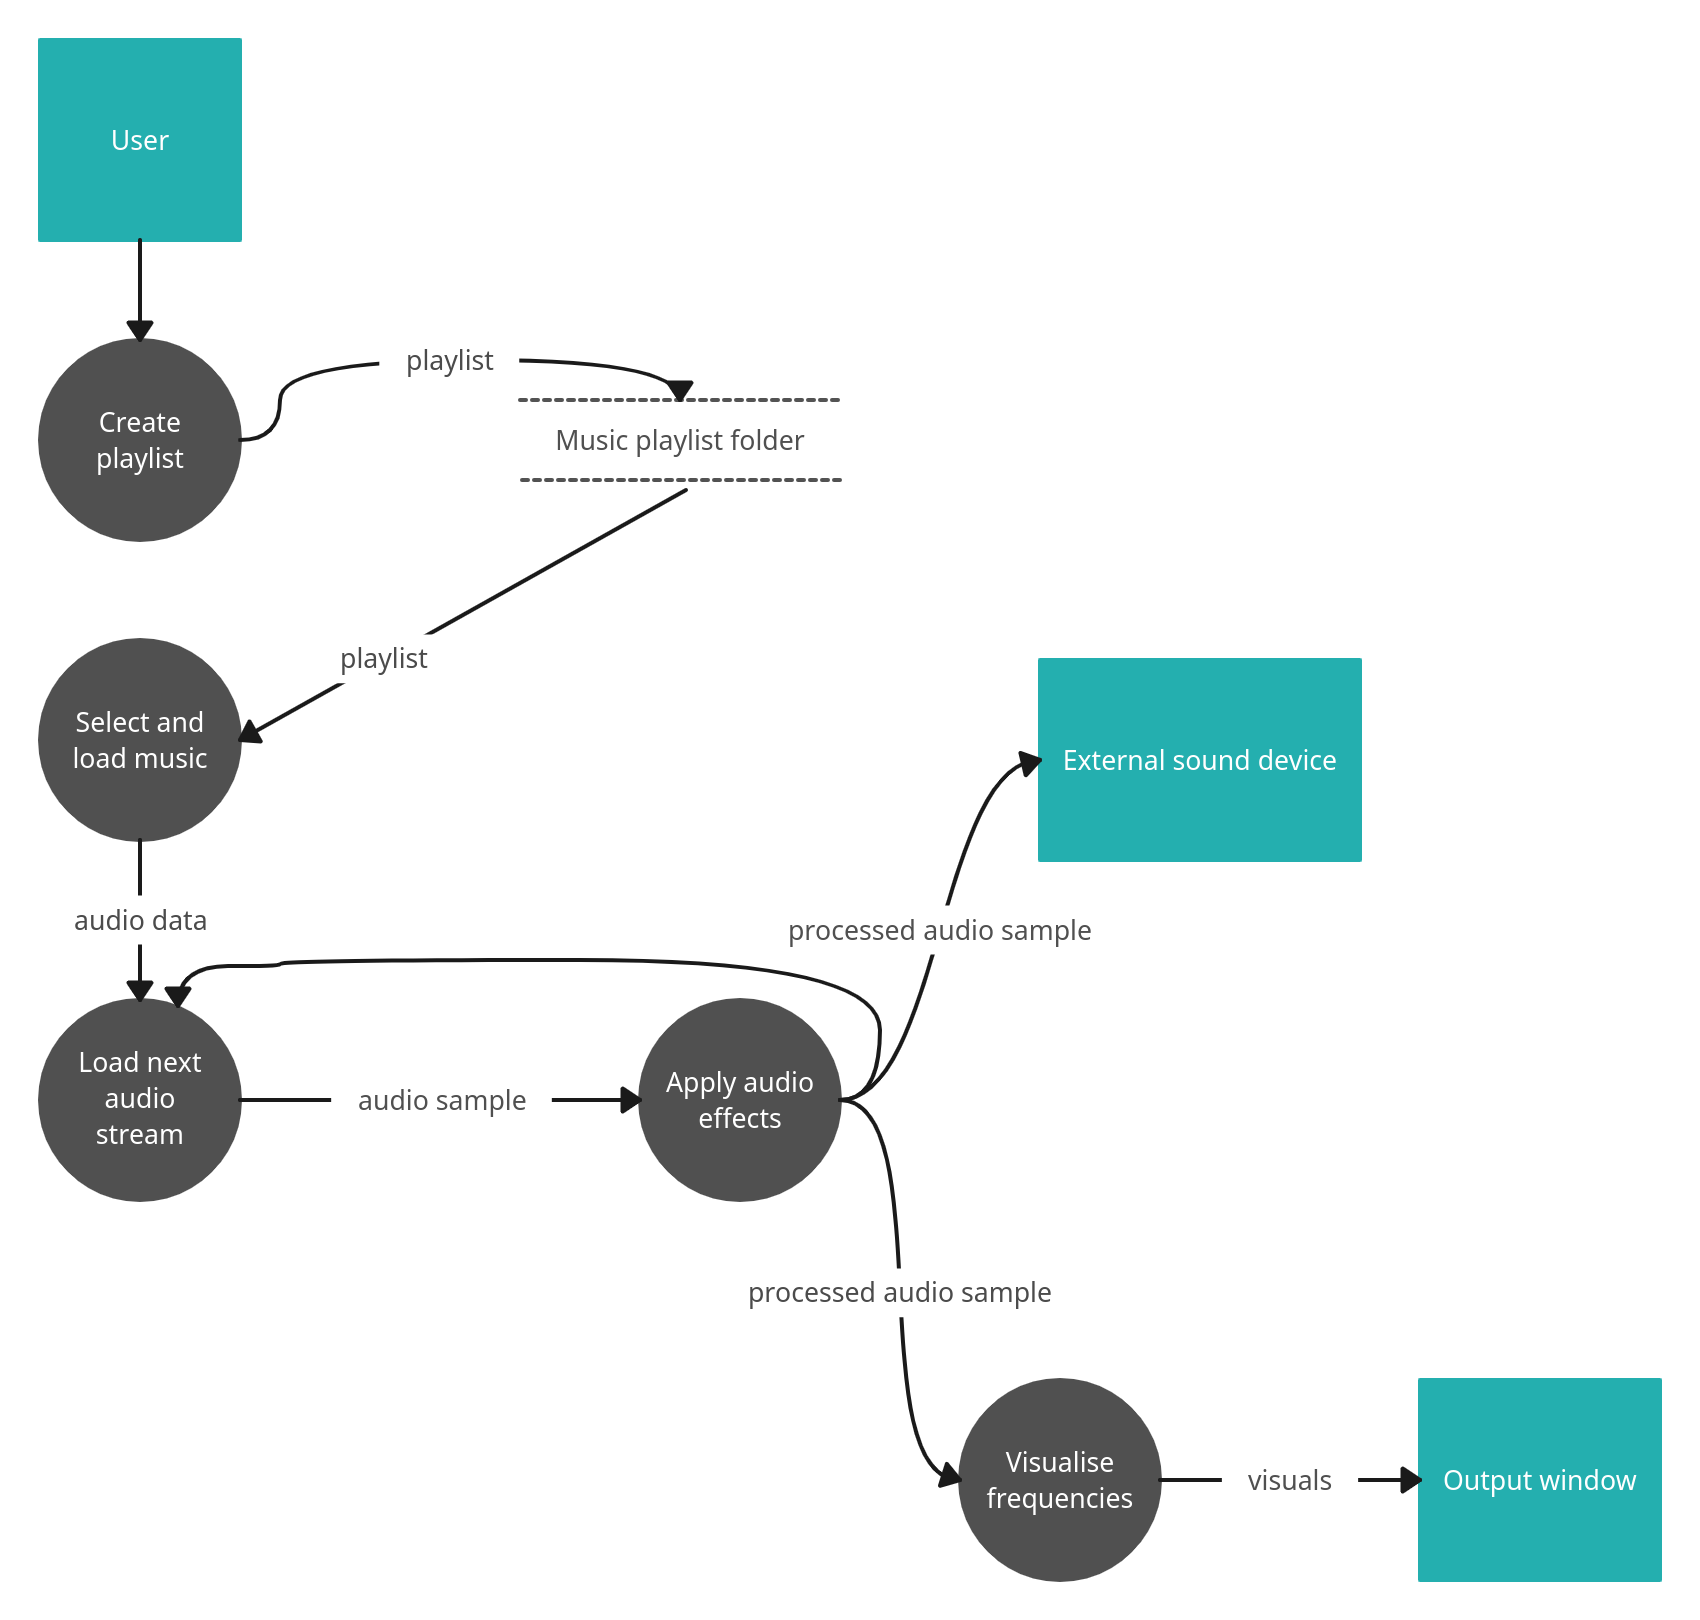
\includegraphics[width=13cm]{DFD}
		\caption{The data flow diagram (DFD)}
	\end{figure}

	\subsection{Analysis of Similar Software Products}
	Every consideration must be given to the existence of other software products which may implement, either partially or fully, the features of the program yet to be implemented.
	
	\paragraph{}
	There exists two broad categories of software which provides features similar to this project:
	\begin{itemize}
		\item Real-time music players - the majority of music listeners listen to music in real-time using streaming services such as Spotify or Apple Music, which can provide certain features to adjust songs in frequency-space (albeit crudely)
		
		\item Audio editors - for those who wish to radically alter audio (e.g. to create a remix), software such as Audacity provides many effects and processing opportunities. These are, however, "offline" in the sense that such software is not real-time.
	\end{itemize}
		
	\subsubsection{Streaming Services}
	Currently within the market the two most popular music streaming products are Apple Music, with 88 million customers in 2022, and Spotify, which over 500 million. These allow users to listen to music on-demand, with both providing an "equaliser" feature that allows the user to modify the relative volume of frequencies within a song in real-time. In other words, with both these products one can, for example, perform a "bass boost", which mirrors very closely one of the main aims of this project.
	
	\begin{figure}[H]
		\caption{The Spotify equaliser}
		\begin{center}
			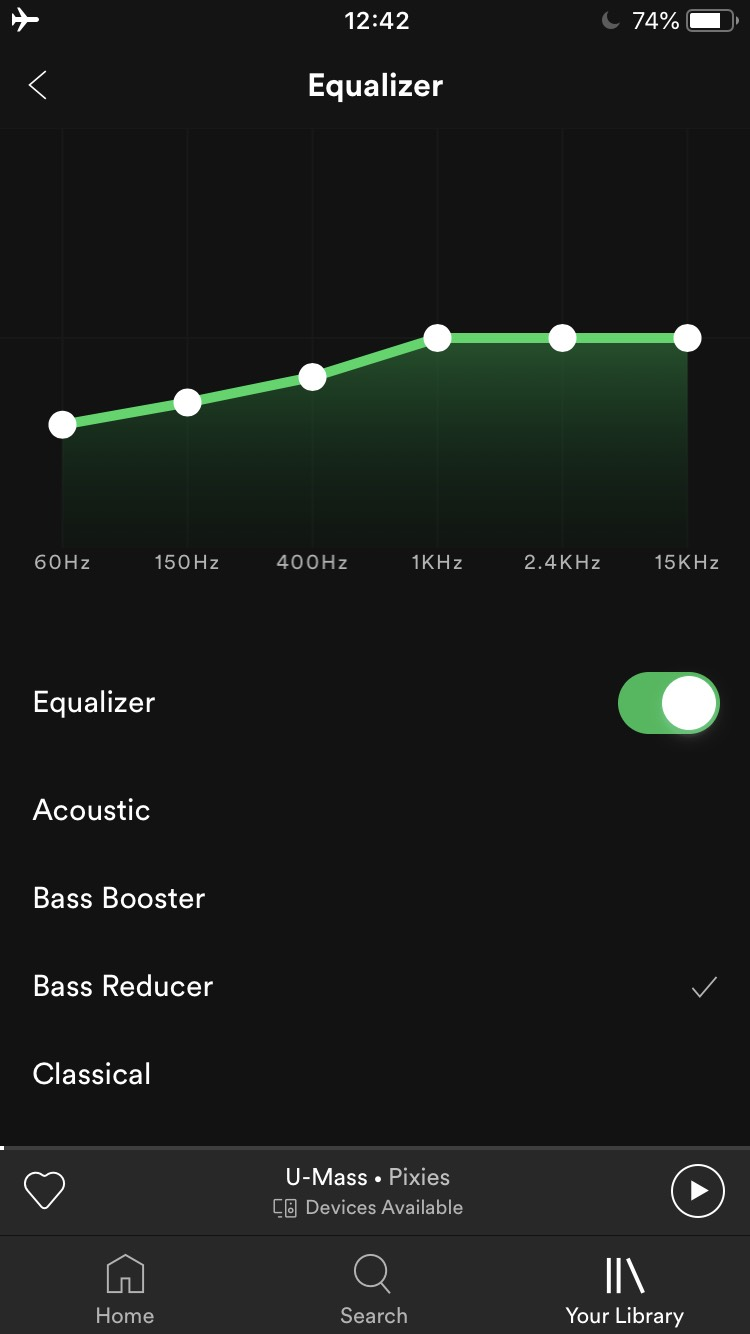
\includegraphics[width=5cm]{spotify equaliser}
		\end{center}
	\end{figure}
	
	\begin{figure}[H]
		\caption{The Apple equaliser}
		\begin{center}
			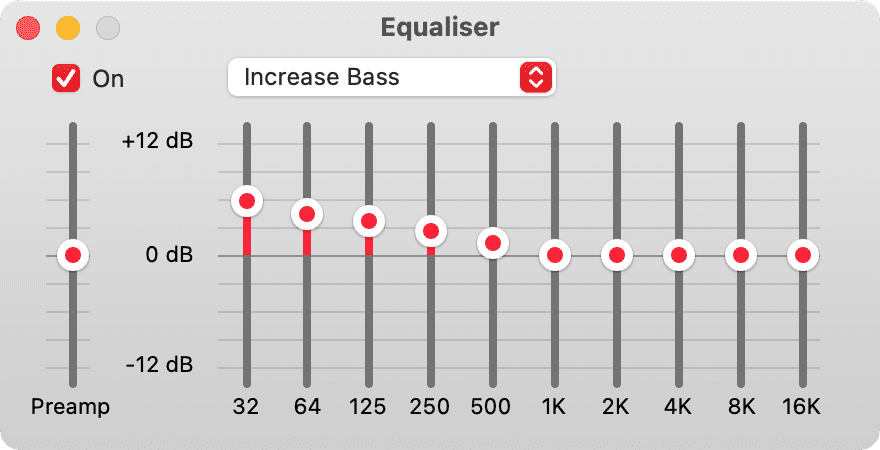
\includegraphics[width=10cm]{apple equaliser}
		\end{center}
	\end{figure}
	
	As can be seen above, there are a number of similarities with the aims of this project:
	\begin{itemize}
		\item The user can easily drag various points  to modify the relative volumes of a number of "frequency groups". For example, one could drag the left-most dot to its maximum height in both to boost frequencies under either 60 or 30 Hz.
		\item Ready-made "presets" can be chosen at will to assist those who may be unfamiliar with the settings presented or want to achieve a particular, pre-made effect.
		\item In Apple Music, the overall volume of the music can be adjusted.
	\end{itemize}
	
	\paragraph{}
	However, there are also a few notable areas in which the two products above fall short of the features being implemented in this project, and hence fail to satisfy the needs of the users outlined in section 1.1.
	\begin{itemize}
		\item In neither case does the user have exact control over the precise frequencies being modified.  If, for example, one had identified a particularly intriguing instrument playing from 500 Hz - 700 Hz, it would be impossible to isolate that frequency and boost it.
		\item There is no option to apply other audio effects such as an echo or noise. As such there are very few ways one can actually modify the audio, so creating a full "remix", that feels distinct from the original, is impossible.
	\end{itemize}

	\paragraph{}
	Thus whilst on a surface-level, the presence of "audio equalisers" in both software products may appear to conflict with the aims of this project, especially as they perform their processing in real-time, closer inspection reveals that they offer only extremely limited options, without the ability to customise which precise frequencies are adjusted or indeed apply any other audio effects.

	\subsubsection{Audio Editing Software}
	On the other hand, there exists many programs which allow a user to modify audio using a great range of effects and filters. As the aim of this project is to lower the barrier of entry to creating song "remixes", it is to be free, and as such it is most worthwhile only considering other free audio editing software.
	
	\paragraph{}
	The most popular free audio editing application is Audacity, an open-source project that supports an extremely large number of effects. Additionally, it supports viewing a spectrogram of the audio being played (which visualises the audio in frequency-space just like this project aims to do), although the feature is somewhat hidden away.
	
	\begin{figure}[H]
		\caption{Audacity when configured to display a spectrogram of the audio, seen as two multi-coloured strips (one for each channel)}
		\begin{center}
			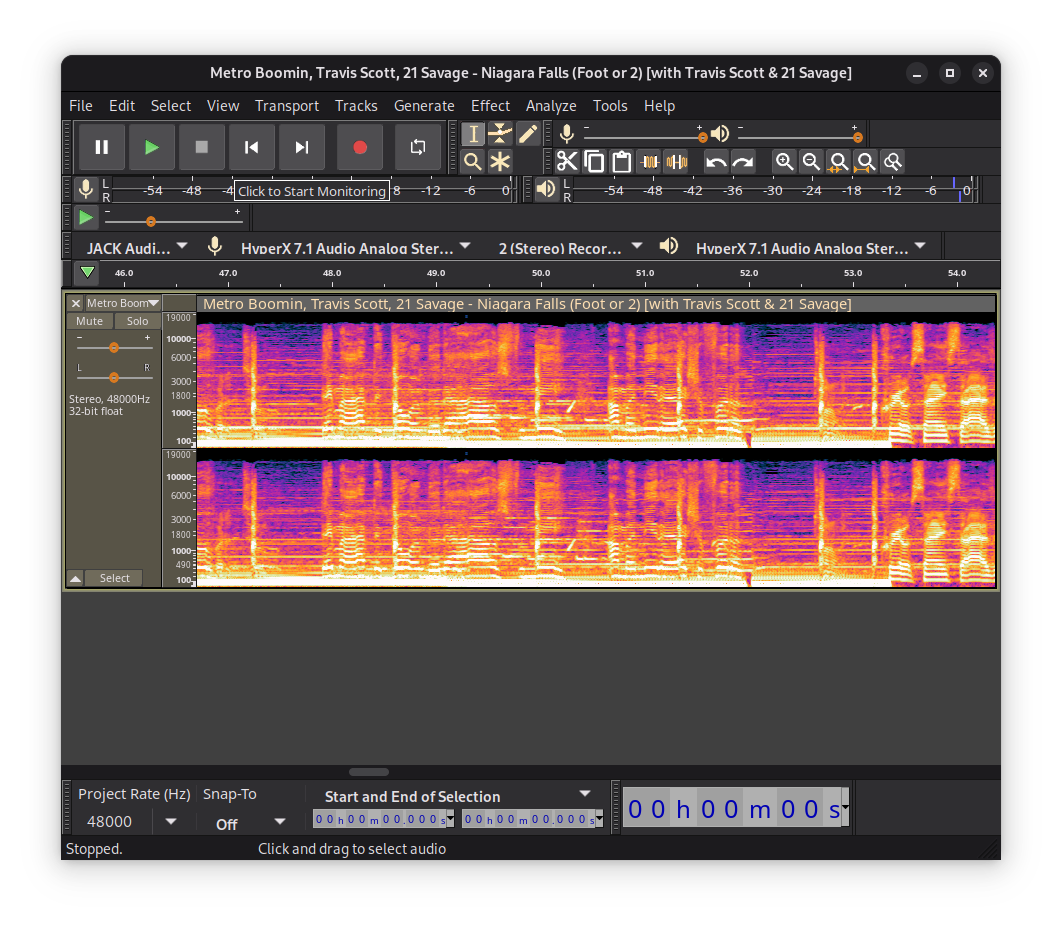
\includegraphics[width=15cm]{audacity spectogram}
		\end{center}
	\end{figure}
	
	\begin{figure}[H]
		\caption{Audacity's "effects menu", offering a number of categories which themselves all contain numerous effects}
		\begin{center}
			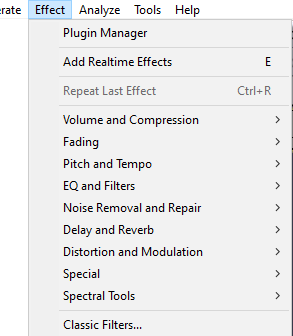
\includegraphics[width=5cm]{audacity effects menu}
		\end{center}
	\end{figure}
	
	\begin{figure}[H]
		\caption{Audacity offering a menu to configure the application of a computationally-intensive, though highly accurate, reverb effect}
		\begin{center}
			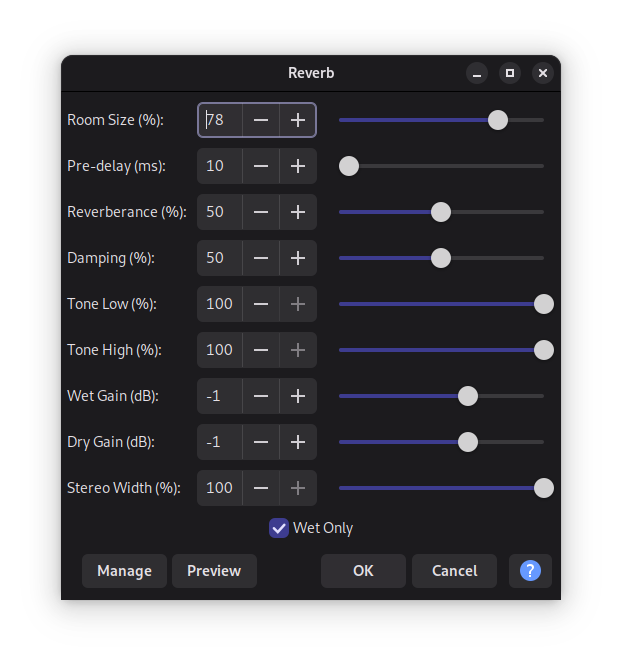
\includegraphics[width=9cm]{audacity effects}
		\end{center}
	\end{figure}
	
	\paragraph{}
	As can be seen above, Audacity thus presents a number of strengths which could be seen to risk overshadowing this project:
	\begin{itemize}
		\item A great number of effects are supported, far greater than this project's scope could hope to provide
		\item The effects are all highly physically accurate, with extreme levels of customisation
	\end{itemize}
	
	However, its weaknesses should also be stressed:
	\begin{itemize}
		\item The user interface is daunting for new users, raising the barrier of entry. For example, the process of displaying a spectrogram is not at all obvious and is hidden away.
		\item The sheer number of parameters for controlling effects is likely very daunting for people that just want a "quick remix".
		\item There are no ready-made "presets" for those too confused to immediately start applying effects themselves, or for those quickly looking for a specific modification.
		\item One cannot apply any effects in real-time, and often the effects are so computationally expensive that one must wait multiple seconds before hearing the result, even on powerful hardware.
		\item It is impossible to create a "music playlist" to listen to multiple songs in quick succession.
	\end{itemize}
	
	Hence it can be seen that whilst Audacity, and other audio editing software, provides many mechanisms for manipulating audio, it cannot be done in real-time, and often powerful hardware is required. They are also completely unsuitable as real-time music players, as they cannot play "playlists". Additionally, the sheer range of editing options would likely prove daunting to even the most experienced user, and so when one considers the high barrier of entry, the failure to be real-time, and the lack of "playlist" functionality, it is clear that audio editing programs such as Audacity do not conflict with the aims of this project.

	\subsubsection{Summary of Similar Software Products}
	\begin{figure}[H]
		\caption{S.W.O.T diagram for streaming services}
		\begin{center}
			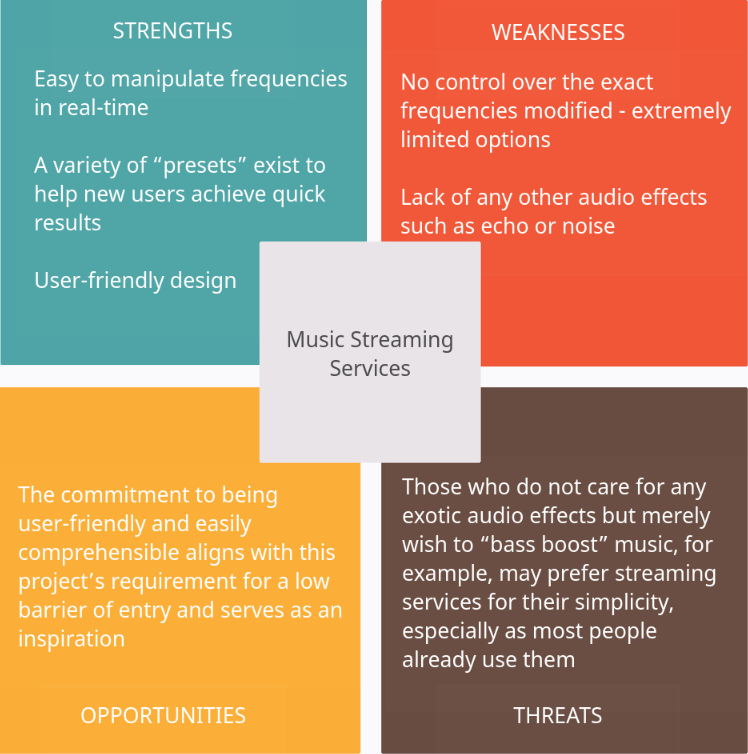
\includegraphics[width=10cm]{SWOT streaming}
		\end{center}
	\end{figure}
	\begin{figure}[H]
		\caption{S.W.O.T diagram for audio editing prograrms}
		\begin{center}
			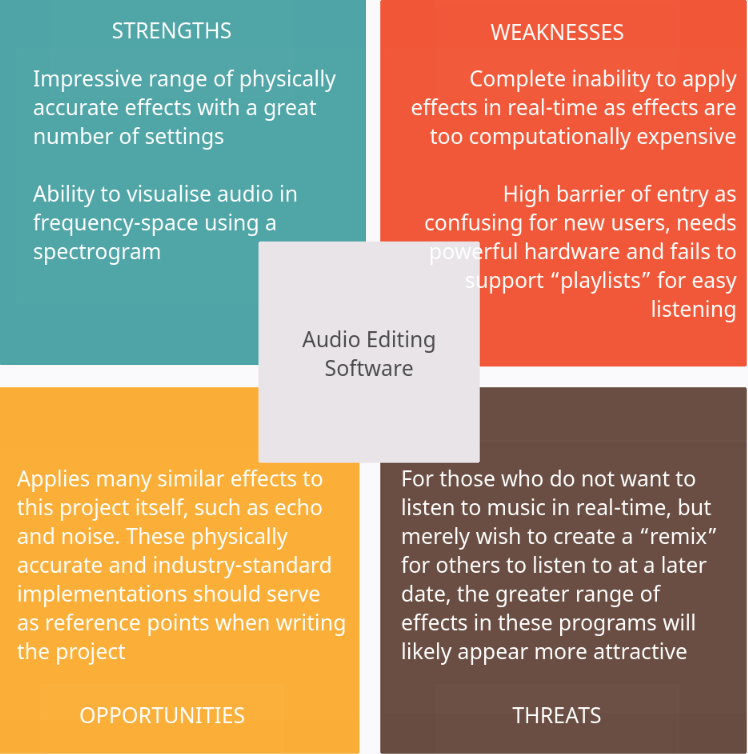
\includegraphics[width=10cm]{SWOT audacity}
		\end{center}
	\end{figure}

	\subsection{Final objectives}
	\begin{enumerate}
	\item  The user must be able to load a collection of audio files known as a "playlist" and then play the audio files contained within in a logical order
	\item  The user must be able to visualise the current audio being played in the frequency domain (i.e. visualise the frequencies)
	\item The user must be able to modify the audio's frequency domain (i.e. selectively modify frequencies such as by performing a bass boost) in realtime
	\item The user must be able to apply additional "audio effects" to further enhance the music: echo, volume adjustment and noise
	\item The user must be able to configure these "audio effects" individually and also apply pre-made "presets" to quickly reach a desired effect
	\item  The system must run in real-time on an average school computer
	\end{enumerate}


	\section { Design }
	
	\subsection{Audio Effects Data Structure}
	The user will likely want to adjust the order of audio effects at will, and as the same time, it must be very fast to insert and  remove audio effects so as to minimise the time spent not processing audio (even a very short pause may result in "crackles" on weaker hardware). To solve this problem, the audio effects can be stored in a linked list, as unlike std::vectors (dynamic C++ arrays) they prove fast insertion, deletion and re-ordering.
	
	\paragraph{}
	To satisfy the requirements of multithreading (see below), I will write my own custom "atomic linked list", backed by a mutex\footnote{
		A mutex is an object that prevents multiple threads from accessing data at the same time. It can be thought of as a lock, which can only be unlocked for one thread at a time. They are preferable to spinlocks as they do not require the CPU to waste cycles waiting for the data to be "unlocked", as instead the thread can suspend itself until the mutex becomes available.
	}, which will function just like a normal linked list but be thread-safe in all its operations.
	
	\subsection{Multithreading}
	In order to maximise ease-of use, the software should have a graphical user environment (GUI) so that the current audio being played can be easily visualised (in-line with objective 2). 
	
	\paragraph{}
	The program will use a multithreaded model, with a separate "audio thread" and "GUI thread", allowing the two to run concurrently without blocking each other's processing. 
	
	\begin{figure}[h]
		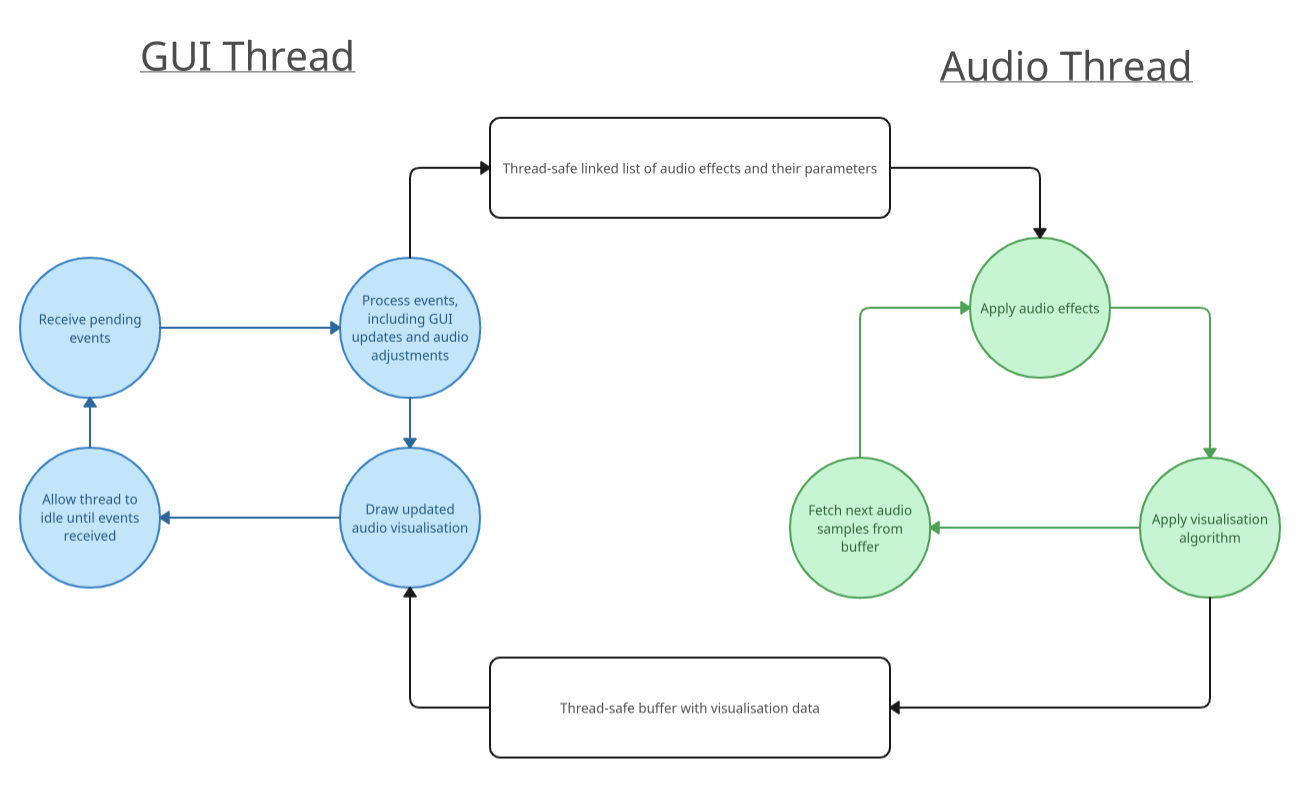
\includegraphics[width=17cm]{threading}
		\caption{Inter-thread diagram}
	\end{figure}
	
	\paragraph{}
	Typically, GUI programs are written using an event-based paradigm that minimises CPU idle-time. The consequence of this is that, for most of the time, the GUI thread is suspended, awoken only when events from the user (such as mouse clicks or resizing the window) "wake it up". This is desirable in order to minimise system resources used, as more CPU-time will be available for the audio processing requirements, helping to reach the real-time requirements of objective 6. However, this presents a unique challenge. With a single-threaded model:
	\begin{itemize}
		\item If the event-based model is followed, the GUI thread is only active when there are pending GUI events to be processed, meaning audio processing can only occur sporadically (resulting in "non-constant" audio)
		\item If instead the GUI thread is constantly active processing audio it will never reach a point where it can process pending events, meaning the program will hang and refuse to process inputs.
	\end{itemize}
	
	Hence it is desirable to split the program into two distinct threads - the "audio thread" and the "GUI thread". The audio thread can play the audio and perform all necessary processing tasks, whilst the GUI thread can relay input parameters and commands to the audio thread (such as "switch song", "apply effect", etc.).
	
	\paragraph{}
	To avoid race conditions\footnote{
		 Race conditions occur when one thread tries to read data whilst the other writes to it. If, for example, the GUI thread removed an audio effect from the audio effect list (see section 2.1) and freed it from memory whilst the audio thread was applying that same effect, the audio thread would suddenly be reading from invalid memory, likely resulting in a crash or undefined behaviour.
	}, the data that is read by both threads should be thread-safe - only one thread should be able to access the data at a time. This can be achieved by using mutexes\footnote{See above footnote on mutexes}.
	
	\section {  Testing }
	
	\section {  Evaluation }
	
	\section { Appendix  }
	
	\subsection{Copy of Interview Questionnaire}
	
	\centering
	\fbox{\begin{minipage}{15cm}
			\begin{center}
			{\huge Luka's Questionnaire Form}
			\end{center}
			
			For my A-level Computer Science coursework  I am writing a program that allows users to easily apply various audio effects to songs, in order to make experimenting with music and creating remixes easier. In order to create the best possible software, I would like your opinion on what makes a remix good. Please answer the questions below in a concise and understandable manner, then email me your responses.
			
			\paragraph{Questions}
			\begin{enumerate}
				\item Why do you sometimes prefer a song's remix?
				\item How does a remix typically differ from the original song?
				\item What features would you like in a real-time audio editing program to assist in "remixing" music?
			\end{enumerate}
	\end{minipage}}
	

	\section { Code example }
		\begin{minted}{c++}
void EqualiserEffect::ModifySamples(std::vector<float>& samples, const float frequency) const
{
	// Perform FFT to convert to frequency domain
	FastFourierTransform fft(samples, std::nullopt);
	std::vector<std::complex<float>>& fft_output = fft.output;
	
	ModifyFrequencies(fft_output, frequency);
	
	// Perform IFFT to convert back to time domain
	InverseFourierTransform inverse(fft_output);
	std::vector<float> scaled_real_components;
	scaled_real_components.reserve(samples.size());
	for (const auto& c : inverse.output)
		scaled_real_components.emplace_back(
			c.real() / (float)inverse.output.size()
		);
	
	samples = scaled_real_components;
}
	\end{minted}
	
	
\end{document}